
\documentclass{article}
\usepackage[utf8]{inputenc} % 支持 UTF-8 编码
\usepackage{ctex}
\usepackage{amsmath}        % 数学公式支持
\usepackage{graphicx}       % 图片插入支持
\usepackage{geometry}       % 页面布局调整
\usepackage{lipsum}
\usepackage{tabularx}
\usepackage{xcolor} % 设置颜色
\usepackage{booktabs} % 提供美观的表格线条
\usepackage{array}    % 提供增强的列格式支持
\usepackage{multirow} % 支持多行合并单元格
\usepackage{makecell} % 支持单元格内容换行
%\usepackage[style=authoryear,backend=biber]{biblatex}
\usepackage{tikz}
\usetikzlibrary{shapes,arrows.meta,positioning}
\usepackage[
colorlinks=true,          % 是否显示颜色而不是边框
linkcolor=blue,           % 内部链接颜色(如目录、交叉引用)
citecolor=red,            % 引用颜色
urlcolor=blue             % URL 颜色
]{hyperref}
\geometry{a4paper, margin=1in} % 设置页面边距


%\addbibresource{refs/references.bib} % 加载参考文献文件


\begin{document}
\pagenumbering{roman} % 设置页码为罗马数字
% 封面

% 封面页
\begin{titlepage}
	\centering

	% 校徽
	
\includegraphics[width=0.6\textwidth]{img/SZU_logo.png} \\
	\vspace{0.5cm} % 校徽与标题之间的间距
	
	% 标题
	\LARGE\bfseries
	综合论文题目: \\
	\vspace{0.5cm} % 标题与副标题之间的间距
	
	% 副标题
	\large\bfseries
	从太赫兹成像到太赫兹无线通信,以及相关技术探究 \\
	\textit{(高新技术讲座课程论文)} \\
	
	\vspace{2cm} % 副标题与正文信息之间的间距
	
	% 正文信息
	\begin{tabular}{l l}
		系别: & 计算机科学与技术系 \\
		专业: & 计算机科学与技术 \\
		学号: & 2025010426 \\
		姓名: & Carroll Polo \\
		指导教师: & Miller  \\
		副指导教师: & Aerith  \\
	\end{tabular}
	
	\vfill % 填充剩余空间到页面底部
	
	% 日期
	\large
	二〇二五年四月 \\
\end{titlepage}



	


%\maketitle

% 学位论文指导小组、公开评阅人和答辩委员会名单
% 本科生不需要
%\input{data/committee}

% 使用授权的说明
% 本科生开题报告不需要
%\copyrightpage
% 将签字扫描后授权文件 scan-copyright.pdf 替换原始页面
% \copyrightpage[file=scan-copyright.pdf]
%\frontmatter

% 中英文摘要和关键字
% 中文摘要
\renewcommand{\abstractname}{摘要} % 将 abstract 标题改为“摘要”
\begin{abstract}
  本文深入探讨了太赫兹技术的定义、原理、特点及其在现代社会中的重要意义。首先介绍了太赫兹的基本概念和核心技术构成,随后分析了太赫兹技术对6G通信组网的潜在影响。并进一步剖析了太赫兹领域中在2018-2025年的重要研究成果,面临的技术挑战。最后,通过分析太赫兹在不同领域的应用实践,展望了太赫兹技术的未来发展趋势。

\end{abstract}

% 中文关键词
\noindent \textbf{关键词:} 太赫兹通信, 6G技术, 脉冲时域成像技术,基于微型石墨烯贴片的天线

\addcontentsline{toc}{section}{摘要} % 将摘要添加到目录中

\newpage

\renewcommand{\abstractname}{Abstract} % 恢复为默认的“Abstract”
\begin{abstract}
	This paper delves into the definition, principles, characteristics, and significance of terahertz (THz) technology in modern society. It first introduces the basic concepts and core components of THz technology, followed by an analysis of its potential impact on 6G network deployment. The paper further examines key research achievements and technical challenges in the field of THz technology from 2018 to 2025. Finally, by exploring practical applications of THz in various fields, it envisions future development trends of the technology.

\end{abstract}

% 英文关键词
\noindent \textbf{Keywords:} Terahertz Communication, 6G Technology, Pulse time domain imaging technology,Antennas based on tiny graphene patches

\addcontentsline{toc}{section}{Abstract} % 将摘要添加到目录中

\newpage

\tableofcontents % 目录
%\addcontentsline{toc}{section}{abstract}
%\addcontentsline{toc}{section}{Abstract}

\clearpage % 强制开始新页,将目录与正文分开
% 插图和附表清单
% 本科生的插图索引和表格索引需要移至正文之后、参考文献前
% \listoffiguresandtables  % 插图和附表清单(仅限研究生)
%\listoffigures           % 插图清单
%\listoftables            % 附表清单
\pagenumbering{arabic} % 阿拉伯数字
% 符号对照表
%\input{data/denotation}


% 正文部分
%\mainmatter

\section{引言/Introduction}

Edholm带宽定律指出,无线通信的带宽需求每隔18个月翻一倍,预计2030年无线传输的峰值速率将超过Tbit/s量级,日渐趋近于有线传输的容量水平。如今5G 使用非常高的毫米波频段,但是 6G 计划使用 100 GHz以上的更高频率,以便满足相较于 5G NR 而言更高的数据传输速率和更低的延迟需求。
如图所示,太赫兹频段(0.1-10THz)介于微波与红外之间,具有丰富的频谱与带宽资源,能够支持实现Tbit/s量
级的传输速率。

\begin{figure}[htbp]
	\centering
	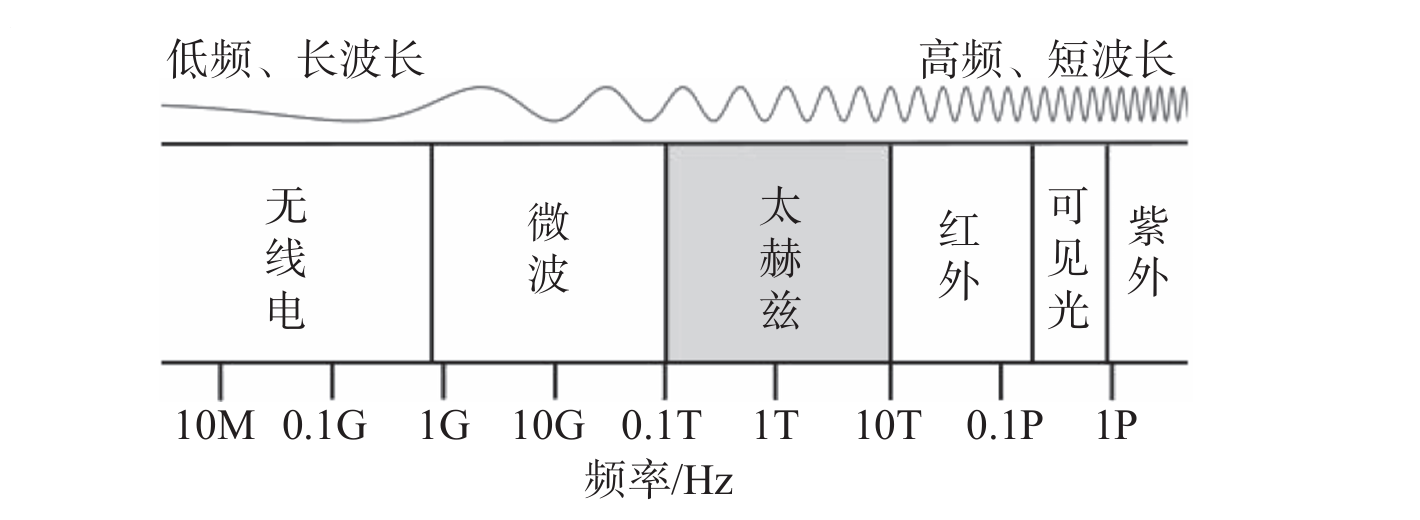
\includegraphics[width=0.6\textwidth]{img/img1.png} % 图片文件名,不需要加扩展名
	\caption{太赫兹频段示意图 \cite{chen2019artificial}}
	\label{fig:example}
\end{figure}

因此,太赫兹通信是 6G 的技术要素之一,其他技术要素包括通信感知一体化 (ISAC)(也称联合通信和传感 (JCAS))、AI 和 ML 以及可重构智能超表面 (RIS)。6G 通信还将使用当前 5G 网络支持的所有频率,例如毫米波频率和传统的 Sub-8 GHz 频段。\\

本文研究了太赫兹成像和太赫兹无线通信技术,重点介绍了这些领域的主要成就和最新进展,确定了它们的相似性和差异,以便更好地理解和探索这些技术。此外,本文还讨论了这两种技术的整合,强调了面临的挑战,并提出了未来的发展方向。本文的其余部分安排如下:第2节介绍了太赫兹技术的基础知识,重点是辐射特性和信号生成;第3节回顾了太赫兹成像技术从过去到现在的发展,包括其主要方法、成就和挑战;第4,5节讨论了太赫兹无线通信,包括其设计架构、技术现状、主要挑战和可能的解决方案,其中重点叙述了基于微型石墨烯贴片的天线,该天线在太赫兹频域具有谐振功能;第6节对两种技术进行了比较,讨论了两种技术整合的可能性,并给出了结论和未来的展望。








\section{太赫兹基础知识}

由于太赫兹波处于电子学(微波)向光子学(红外,可见光)过渡的阶段,因此它同时具备了微波通信和光通信的优点。有两种方法可以产生太赫兹波:一种是使用电子源将频率增加两倍或三倍,达到所需的太赫兹频率;另一种是使用一个或多个光学源,将信号变频到所需的太赫兹频率。这两种方法都不是很有效,而且产生的太赫兹信号通常很小(小于10 mW),这限制了它的应用。


\subsection{太赫兹的传播特性}

与射频和微波一样,太赫兹波是非电离且非破坏性的,从本质上来说,对人类是安全的。然而,太赫兹波的波长更短[1THz的波长是0.3 mm(300.0 μm)],因此能够提供比微波更高的成像分辨率。虽然它们对大多数材料的穿透深度不如微波,但它比红外和可见光的穿透深度要好,可以显示身体和包装中的隐藏物体。无线电P传播的路径损耗(Lp)是无线通信和成像的一个主要参数,由Friis公式\cite{huang2021antennas}控制

\begin{equation}
	L_{\mathrm{p}} = 10 \times \lg \left( \frac{P^{\mathrm{t}}}{P^{\mathrm{r}}} \right) = 20 \times \lg f + 20 \times \lg r - 147.6 \ (\text{in dB})
	\tag{1}
\end{equation}

其中,Pt是发射器功率;Pr是接收器功率;f是频率;r是距离。我们可以看出,路径损耗与频率f的平方和距离r的平方成正
比。频率越高,路径损耗就越大。除此以外,太赫兹波受大气频率选择性吸收,即使对于室内环境,隔断损失也在太赫兹中非常显著。

\begin{figure}[htbp]
	\centering
	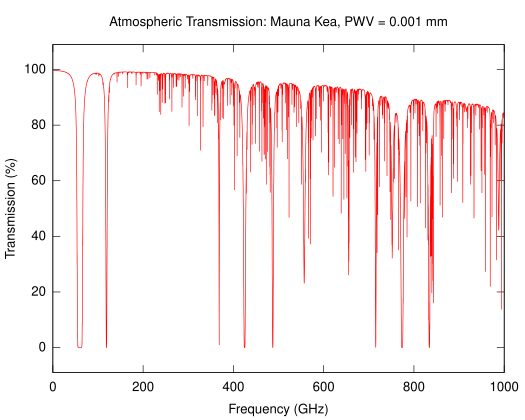
\includegraphics[width=0.6\textwidth]{img/img2.png} % 图片文件名,不需要加扩展名
	\caption{大气太赫兹辐射透射率\cite{982447}}
	\label{fig:example}
\end{figure}



\subsection{太赫兹信号的产生和检测}
目前,太赫兹研究和开发的进展缓慢,主要原因是缺乏太赫兹硬件,特别是缺乏紧凑型和经济型的太赫兹源。

有两种方法可以产生太赫兹波:一种是使用电子源
将频率增加两倍或三倍,达到所需的太赫兹频率;另一种
是使用一个或多个光学源,将信号变频到所需的太赫兹频
率。这两种方法都不是很有效,而且产生的太赫兹信号通
常很小(小于10 mW),这限制了它的应用。

太赫兹检测使用太赫兹探测器,太赫兹探测器是用于检测太赫兹波(频率范围为 0.1 THz 到 10 THz)的传感器,其核心功能是将入射的太赫兹波信号转换为可测量的电信号。由于太赫兹探测器的设计和工作原理受到太赫兹波的特殊性质的影响,例如其较高的频率和较短的波长\cite{10697786}。因此,太赫兹探测器需要具备以下关键性能:

高灵敏度:能够检测微弱的太赫兹信号。
快速响应:能够实时捕捉动态变化的信号。
宽频带:能够在较大的频率范围内工作。
低噪声:减少背景干扰对信号检测的影响。根据工作原理和技术特点,太赫兹探测器可以分为多种类型,包括光电式探测器、热敏型探测器、超导探测器、半导体探测器。具体每种太赫兹探测器已有诸多资料可供查阅,这里不多赘述。


\section{太赫兹成像与传感领域}

第一幅太赫兹图像是由Hartwick等使用光学泵浦
的分子太赫兹激光器得到的。1995年,Hu和Nuss利
用基于飞秒激光源的光电太赫兹成像技术,在太赫兹科学
和技术领域引发了一波研究兴趣和活动。在过去的20年
里,太赫兹成像科学技术在基础研究和实际应用方面都取
得了巨大的进展。

\subsection{脉冲时域成像系统}

脉冲太赫兹TDS的核心技术使用飞秒激光器相干地产生和检测短脉冲。分束器(BS)用于将飞秒脉冲激光的近红外(NIR)光分成两部分:泵浦光束和探测光束。泵浦光束聚焦到一个有偏压的光电导天线表面,用于产生太赫兹。在外加电场下,飞秒激光脉冲在砷化镓晶体中产生的载流子产生瞬时电流,从而产生太赫兹频率的脉冲波。辐射的太赫兹脉冲被收集、准直,然后聚焦到被测样品上\cite{8702204}。

然后,从样品上反射回来的太赫兹脉冲被接收并聚焦到一个无偏压的光电导天线上,用于激光门控太赫兹检测。通常在太赫兹发射/接收天线上连接硅透镜(SL),可以提高太赫兹辐射耦合效率。通过用一个可变延迟电动平台来扫描近红外探测光束,以检测太赫兹脉冲的时间分辨电场。

\subsection{医疗和生物应用}

太赫兹辐射具有较低的光子能量(即非电离辐射),不会对人体造成任何安全风险。然而,它会因受到水的影响而强烈衰减,因此,太赫兹辐射对水含量非常敏感。在过去的10年里,人们对太赫兹光谱和成像在生物和医疗方面的应用越来越感兴趣。

2018年,Jung等使用太赫兹技术对早期宫颈癌患者淋巴结进行检测,实验对在体癌症引流区域的淋巴结进行分析成像,与术后淋巴结病理检查结果进行比较,结果发现淋巴结转移区域的反射峰振幅与正常淋巴结区域的反射峰振幅相比明显降低,太赫兹光谱成像能够显示最小约3 mm转移灶的轮廓。皮瓣是从人体健康处取下,带有血液供应的组织,其能否存活于损伤部位是皮瓣移植手术成功与否的关键。Bajwa及其同事将6只小鼠背部取得的皮瓣分成2组:皮瓣存活组和皮瓣坏死组(由组织学证实),使用太赫兹成像技术动态监测了一周内两组皮瓣含水量的变化,结果表明,太赫兹成像可以先于肉眼观察24h发现两组皮瓣的变化。Bajwa等的另一项研究同样是基于水含量的变化来探讨太赫兹成像对比(magnetic resonance imaging,MRI),从而来评估烧伤程度,这是首次体内评估太赫兹成像的水含量对比度和探测深度。此外,Hernandez-Cardoso及其同事将太赫兹成像技术在糖尿病的早期诊断中进行了测试。其中糖尿病组12人、对照组21人。受试者坐在特定的装置上,对足底进行太赫兹成像,分别比较了大拇趾、足底中部和脚后跟的数据后,结果均显示糖尿病组皮肤组织中水含量明显少于对照组,如图3所示。

\begin{figure}[htbp]
	\centering
	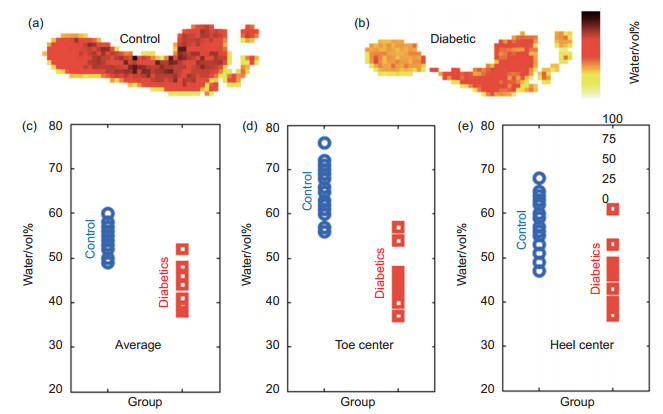
\includegraphics[width=0.6\textwidth]{img/img4.jpg} % 图片文件名,不需要加扩展名
	\caption{糖尿病足组与对照组的水含量的比较。(a)对照组太赫兹成像图;(b)糖尿病足组太赫兹成像图;(c)足底水含量;(d)拇趾中心水含量;(e)脚后跟中心水含量\cite{hernandez2017terahertz}}
	\label{fig:example}
\end{figure}
\section{太赫兹无线通信}

根据太赫兹信号的产生方式不同,太赫兹通信系统可分为基于电子学和基于光子学两类,基于光子学的太赫兹波产生方法又细分为光子辅助型和量子级联型 \cite{deng2022terahertz}.

上述分类方式仅为众多分类方式中的一种,还包括 按照频段划分(如低频,高频太赫兹通信),按照通信模式划分(点对点通信系统 广播通信系统 移动通信系统),按照应用场景划分。下述为以发射与接收技术划分的太赫兹无线通信方式。

\subsection{全电子型}

传统基于电子学的太赫兹通信系统的发射端一般由基带和射频前端两部分构成。数据域基带信号通常在能够进行高速计算的现场可编程门阵列(fieldprogrammable gate array, FPGA)上完成处理,随机信源序列在经过加扰、编码与调制后实现到基带信号
的转换,如图3(a)所示。前端部分则由基带系统、倍频器、混频器、本征信号源、功率放大器以及天线等组成,其结构如图3(b)所示。基带产生的数字信号经由数模转换器(digital to analog converter, DAC)处理后,转换为中频模拟信号。

\begin{figure}[ht]
	\centering
	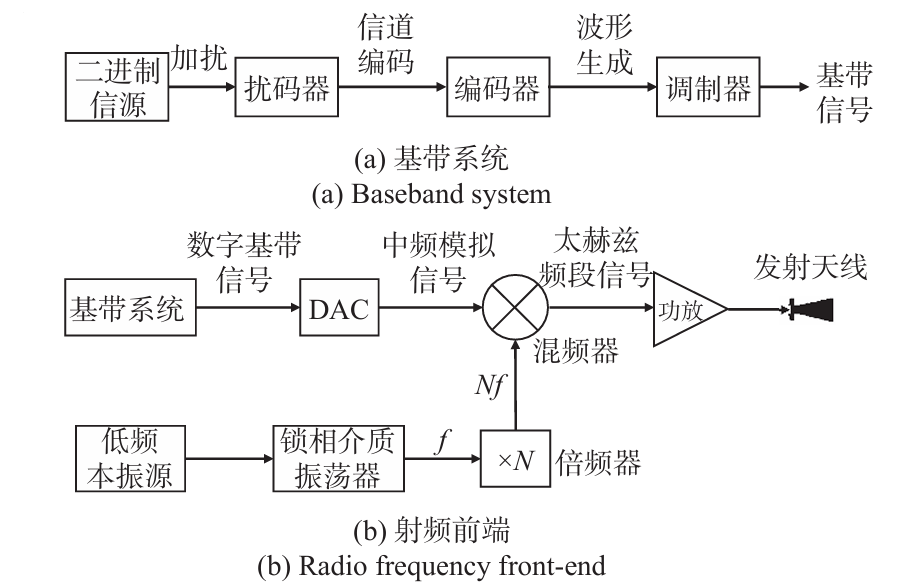
\includegraphics[width=0.6\textwidth]{img/img3.png} % 图片文件名,不需要加扩展名
	\caption{基带信号与射频前端 \cite{shi2024terahertz}}
	\label{fig:example}
\end{figure}

在射频部分,低频的本振信号依次经过锁相介质振荡器和倍频器后,被搬移到高频段。随后,混频器取倍频后信号的多次谐波,将中频模拟信号混频到指定的太赫兹频段,所得太赫兹信号经过功率放大器后,最后通过天线发射出去。

全电子型发射端的电子器件体积小、集成度高, 有利于通信系统小型化;发射功率高,可实现较远距 离无线传输。但半导体设计与加工难度受限,利用 倍频器难以产生超高频率(≥1 THz)的太赫兹信 号。此外,调制解调与编译码过程也受到基带信号 处理芯片能力限制,实时传输速率难以达到 $10^{11}$  bit/s量级及以上。


\subsection{光电子型}

得益于太赫兹波段介于微波与红外波之间,凭借其近光性,可以利用光子学方法来生成频率更高,带宽更大的太赫兹信号。由此,科学家设计了光电子型(光电外差拍频型)的太赫兹通信系统。其通过光电转换来产生太赫兹信号,借助光波的超高频率与光学器件的大带宽突破了电子器件带宽受限的问题

光电式太赫兹通信系统的发射端利用飞秒激光脉冲照射半导体材料(如 GaAs 或 InGaAs),通过光电导天线或光整流效应产生太赫兹波。其接收端:用光电导探测器、热释电探测器或肖特基二极管探测器等,将太赫兹信号转换为电信号。光电式太赫兹通信系统具有高分辨率、高灵敏度等优点。但设备复杂,成本较高,通常需要额外的光学系统支持。


\subsection{光量子型}
全电子型和光子辅助型方式产生的太赫兹信号的频率基本不超过1 THz,一般需要用量子级联型(又称直接调制激光型)方式才能产生1 THz以上的太赫兹信号。在该方法中,最常用太赫兹量子级联激光器(terahertz quantum cascade laser, THz-QCL)直接进行高速调制,但该器件对工作环境要求苛刻,需要满足低温条件,极大地限制了量子级联型方式在实际太赫兹通信系统中的应用。

\subsection{总结}
光电式太赫兹通信系统:结合光学和电子技术,具有高分辨率和高灵敏度,但设备复杂且成本较高。
全电子式太赫兹通信系统:完全基于电子学技术,设备紧凑、集成度高,适合远距离传输,但半导体设计难度大。
全光子式太赫兹通信系统:完全基于光学技术,具有高带宽和高灵敏度,适合超高数据速率的应用,但设备复杂且实时性较差。
\begin{table}[htbp]
	\centering
	\caption{太赫兹通信系统分类与对比}
	\label{tab:terahertz_systems}
	\resizebox{\textwidth}{!}{ % 自动缩放到页面宽度
		\begin{tabular}{c c c c c c p{8cm}} % 也可调窄p列
			\toprule
			\textbf{系统类型} & \textbf{信号产生方式} & \textbf{下变频方式} & \textbf{传输距离} & \textbf{系统集成度} & \textbf{光纤集成程度} & \textbf{6G典型适用场景} \\
			\midrule
			全电子型 & 基于电子学 & 全电子学 & 长 & 高 & 难 & \makecell[l]{多频段融合密集网络,通感一体车联网与AD,\\无人机自组网,卫星空间通信,军事保密通信} \\
			光子辅助型 & 基于光子学 & 光电混合 & 短 & 中 & 中 & \makecell[l]{室内XR与HC,数据中心物联网,光纤融合应急网络} \\
			全光子型 & 基于光子学 & 全光子学 & 短 & 低 & 易 & \makecell[l]{近距离探测成像,片上测试与通信} \\
			\bottomrule
		\end{tabular}
	}
%	\caption{Classification and comparison for terahertz communication systems}
\end{table}

\section{太赫兹无线通信的主要挑战}
很明显,最近在电子和光子太赫兹收发器设计方面的进展已经实现了高效的信号生成、调制和辐射。经过审查的大多数太赫兹无线通信系统都低于300 GHz,为了达到大于1Tbps的数据速率,工作频率将高于300~500GHz。根据国际半导体技术路线图(International Technology Roadmap for Semiconductors, ITRS),硅互补金属氧化物半导体(Si-CMOS)的截至频率将在几年内超过500 GHz。但在实际应用中仍面临诸多挑战。以下是太赫兹无线通信面临的主要挑战。

\subsection{传播损耗与功率}

太赫兹波段的电磁波在空气中极易被水蒸气、氧气等分子吸收,导致信号衰减严重。水蒸气对太赫兹波的吸收尤为显著,尤其是在高湿度环境下,信号衰减会进一步加剧。这种吸收效应限制了太赫兹通信的传输距离,通常仅适用于短距离通信场景。目前基于电子的太赫兹系统产生的功率通常低于
10 mW。因此,除非采用高增益天线,否则传输距离非常
短。随着功率和工作频率的提高,功耗和散热可能成为主
要问题,因为导电材料的欧姆损耗与频率成正比,而太赫
兹设备和系统的尺寸必然很小。

\subsection{精密电子器件的制造}

虽然射频/微波设备的制造已经成熟,但太赫兹设备的制造还不成熟。基本的二极管和晶体管在太赫兹波段还不能很好地工作。高精度的机械加工已经生产出许多高质量的毫米波和亚太赫兹天线和波导,但难以满足更高频率的要求。当半导体器件的工作频率高达太赫兹频段,半导体材料的影响和器件封装的分布式参数效应直接影响电路和系统的性能。

到目前为止,2DEG复合材料
(如GaN HEMT)和2D材料(如石墨烯)\cite{10698344}已经被应用于太赫兹调制器。因此,未来可以开发在太赫兹波段响应时
间小于1 ps的人造材料,用于器件的制造。

\begin{figure}[htbp]
	\centering
	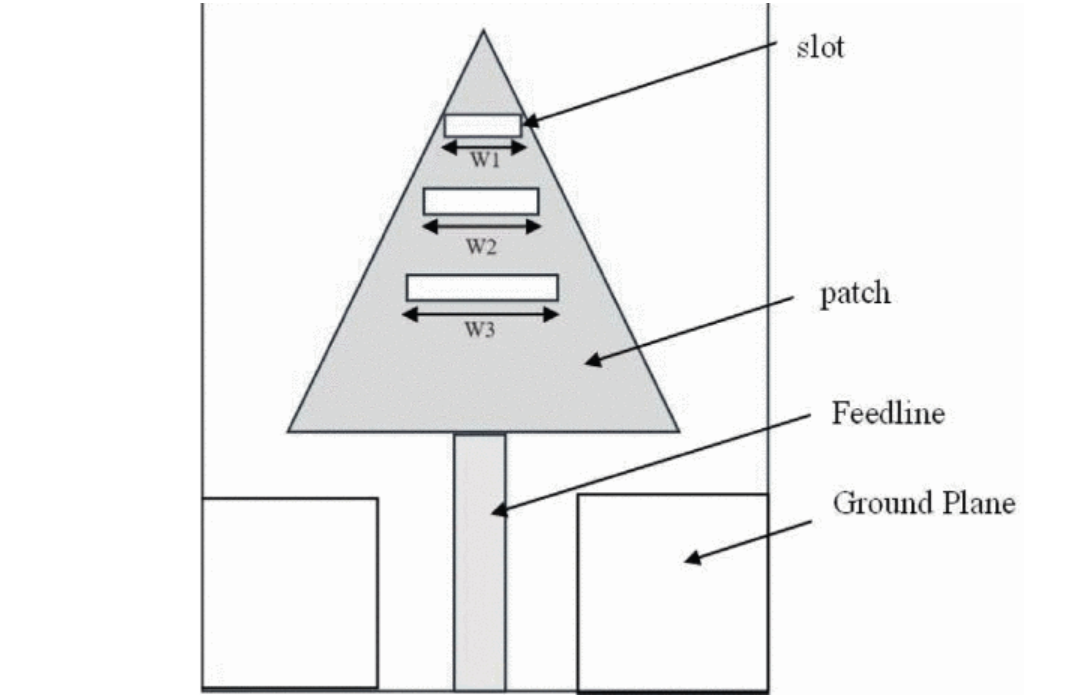
\includegraphics[width=0.6\textwidth]{img/img5.png} % 图片文件名,不需要加扩展名
	\caption{太赫兹频段示意图}
	\label{fig:example}
\end{figure}

如图5所示,
slot为缝隙槽,
patch为贴片,
feedline为馈线,
groud plane为接地平面。

随着缝隙数量的增加,带宽增加,但超过3个缝隙后,带宽开始减小。每个缝隙的宽度和缝隙之间的间距为2μ m。
该贴片采用共面波导 (CPW) 馈线供电,因为它可以降低损耗,使天线结构更加平面紧凑。为了设计谐振频率在 3 THz 附近的等边三角形贴片,可使用以下公式
\begin{equation*} f_{r}=\frac{2c}{3a\sqrt{\varepsilon_{r}}} \tag{2} \end{equation*}
\begin{align*}
	f_{r} &\quad \text{是共振频率,} \\
	\varepsilon_{r} &\quad \text{是基底的相对介电常数,} \\
	a &\quad \text{是三角形面片的边长。}
\end{align*}

该天线由开槽三角形石墨烯贴片组成,并采用共面波导馈电。增加3个缝隙后,带宽显著改善,在3.2至30 THz范围内具有宽带频率响应,即在太赫兹频率范围内表现出超宽带响应。其平面结构、紧凑性和辐射特性使其适用于太赫兹范围内的生物医学、电信和制药行业的各种应用。未来的研究方向包括制造和性能参数测量。
\section{总结与展望/ConclusIon And RecommendAtIons}

本文首先从6G典型应用场景及其性能需求出发,分析了研究巨容量太赫兹无线通信的必要性。接着,概述了6G网络架构和太赫兹在其中的重要作用以及国内外太赫兹通信发展现状。然后,根据太赫兹信号的产生与接收方式阐述了太赫兹无线通信系统的架构与分类。针对太赫兹成像与传感领域,本文重点介绍了脉冲时域成像系统与太赫兹成像技术在糖尿病患者的检测的应用。

THz通信具备高数据传输速率和宽带宽等优点, 信息传输过程中安全性能高, 有望引入6G系统中. 通过探索THz产生新方法、发展新天线技术来提高THz信号的增益,优化系统资源分配, 进而实现小型化、低功耗和低成本的THz通信系统, 增加通信覆盖面, 提升数据传输速率和传输距离, 使6G无线网络为人们提供生活的便利。




% 其他部分
%\backmatter

%\appendix
%\input{data/appendix}
\newpage
% 参考文献

\addcontentsline{toc}{section}{参考文献} % 将参考文献添加到目录中

\bibliographystyle{unsrt}
\bibliography{refs/references}



\end{document}
